\chapter{Recurrent Neural Networks (RNN) (1982)}


\begin{figure}[H]
    \centering
    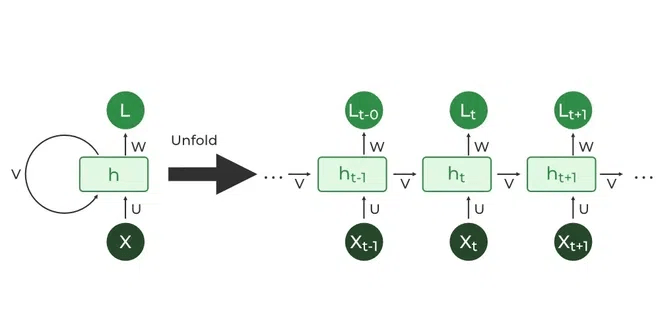
\includegraphics[
        width=\linewidth,
        height=5cm,
        keepaspectratio,
    ]{images/recurrent-neural-networks/Recurrent-Neural-Network_gfg.png}
    \caption{Recurrent Neural Networks: Unfolding \cite{geeksforgeeks/machine-learning/introduction-to-recurrent-neural-network}}
\end{figure}


\begin{enumerate}
    \item Recurrent Neural Networks (RNNs) differ from regular neural networks in how they process information. While standard neural networks pass information in one direction i.e. from input to output, RNNs feed information back into the network at each step.
    \hfill \cite{geeksforgeeks/machine-learning/introduction-to-recurrent-neural-network}

    \item RNNs work by “remembering” past information and passing the output from one step as input to the next i.e it considers all the earlier words to choose the most likely next word. 
    This memory of previous steps helps the network understand context and make better predictions.
    \hfill \cite{geeksforgeeks/machine-learning/introduction-to-recurrent-neural-network}

    \item Recurrent neural networks (RNNs) are a promising architecture for general-purpose sequence transduction.
    \hfill \cite{arxiv/1211.3711/Sequence-Transduction-RNN}

    \item The combination of a high-dimensional multivariate internal state and nonlinear state-to-state dynamics offers more expressive power than conventional sequential algorithms such as hidden Markov models.
    \hfill \cite{arxiv/1211.3711/Sequence-Transduction-RNN}

    \item In particular, RNNs are better at storing and accessing information over long periods of time.
    \hfill \cite{arxiv/1211.3711/Sequence-Transduction-RNN}

    \item RNNs are usually restricted to problems where the alignment between the input and output sequence is known in advance.
    For example, RNNs may be used to classify every frame in a speech signal, or every amino acid in a protein chain. 
    If the network outputs are probabilistic this leads to a distribution over output sequences of the same length as the input sequence. 
    \hfill \cite{arxiv/1211.3711/Sequence-Transduction-RNN}

    \item Unlike traditional feedforward neural networks which process inputs as fixed-length vectors, RNNs can manage \textbf{variable-length sequences} by maintaining a hidden state that stores information from previous steps in the sequence.
    \hfill \cite{geeksforgeeks/deep-learning/bidirectional-recurrent-neural-network}
\end{enumerate}




\section{Key Components of RNNs}

\begin{enumerate}

\begin{figure}[H]
    \centering
    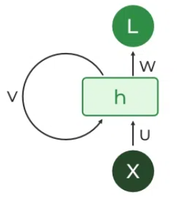
\includegraphics[
        width=\linewidth,
        height=2.5cm,
        keepaspectratio,
    ]{images/recurrent-neural-networks/rnn-gfg-1-recurrent-neuron.png}
    \caption{RNN: Neuron (Recurrent Unit) \cite{geeksforgeeks/machine-learning/introduction-to-recurrent-neural-network}}
\end{figure}

    \item \textbf{Recurrent Neurons} (Recurrent Unit): They hold a hidden state that maintains information about previous inputs in a sequence. 
    Recurrent units can "remember" information from prior steps by feeding back their hidden state, allowing them to capture dependencies across time.
    \hfill \cite{geeksforgeeks/machine-learning/introduction-to-recurrent-neural-network}

\begin{figure}[H]
    \centering
    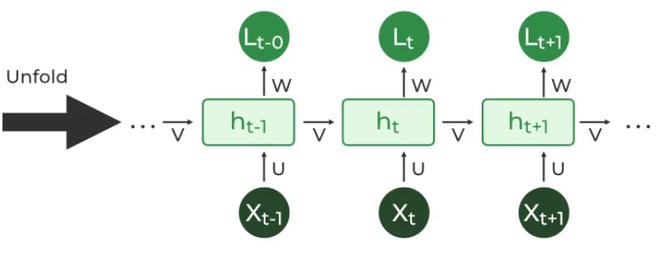
\includegraphics[
        width=\linewidth,
        height=2.5cm,
        keepaspectratio,
    ]{images/recurrent-neural-networks/rnn-gfg-2-Unfolding.png}
    \caption{RNN: Neuron (Recurrent Unit) \cite{geeksforgeeks/machine-learning/introduction-to-recurrent-neural-network}}
\end{figure}

    \item \textbf{RNN Unfolding}: RNN unfolding or unrolling is the process of expanding the recurrent structure over time steps. 
    During unfolding each step of the sequence is represented as a separate layer in a series illustrating how information flows across each time step.
    This unrolling enables backpropagation through time (BPTT) a learning process where errors are propagated across time steps to adjust the network’s weights enhancing the RNN’s ability to learn dependencies within sequential data.
    \hfill \cite{geeksforgeeks/machine-learning/introduction-to-recurrent-neural-network}

\end{enumerate}




\section{How does RNN work?}

\subsection*{Forward Pass}

\begin{enumerate}
    \item \textbf{State Update}: $h_t=f(h_{t-1},x_t)$
    \hfill \cite{geeksforgeeks/machine-learning/introduction-to-recurrent-neural-network}
    \begin{enumerate}
        \item $h_t$ is the current state
        \hfill \cite{geeksforgeeks/machine-learning/introduction-to-recurrent-neural-network}
        
        \item $h_{t-1}$ is the previous state
        \hfill \cite{geeksforgeeks/machine-learning/introduction-to-recurrent-neural-network}
        
        \item $x_t$ is the input at the current time step
        \hfill \cite{geeksforgeeks/machine-learning/introduction-to-recurrent-neural-network}
    \end{enumerate}

    \item \textbf{Activation Function Application}: $h_t=\tanh(W_{hh}\cdot h_{t-1}+W_{xh}\cdot x_t)$
    \hfill \cite{geeksforgeeks/machine-learning/introduction-to-recurrent-neural-network}
    \\
    Here, $W_{hh}$ is the weight matrix for the recurrent neuron and $W_{xh}$ is the weight matrix for the input neuron.
    \hfill \cite{geeksforgeeks/machine-learning/introduction-to-recurrent-neural-network}

    \item \textbf{Output Calculation}: $y_t=W_{hy}\cdot h_t$
    \hfill \cite{geeksforgeeks/machine-learning/introduction-to-recurrent-neural-network}
    \\
    where $y_t$ is the output and $W_{hy}$ is the weight at the output layer.
    \hfill \cite{geeksforgeeks/machine-learning/introduction-to-recurrent-neural-network}

    \item These parameters are updated using backpropagation. 
    However, since RNN works on sequential data here we use an updated backpropagation which is known as backpropagation through time.
    \hfill \cite{geeksforgeeks/machine-learning/introduction-to-recurrent-neural-network}
\end{enumerate}


\subsection*{Backward Pass/ Backpropagation}

\begin{figure}[H]
    \centering
    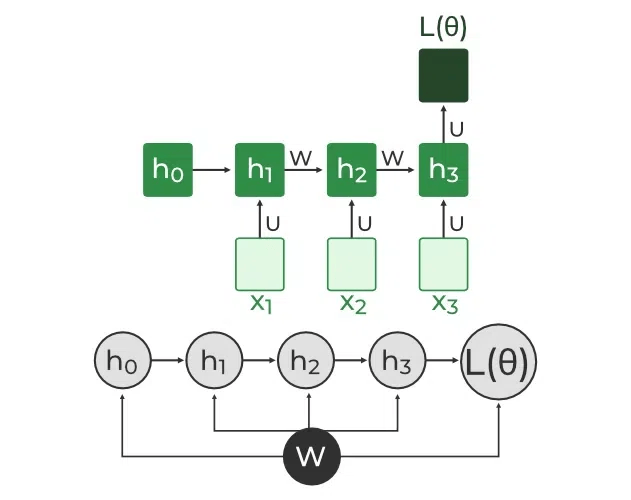
\includegraphics[
        width=\linewidth,
        height=5cm,
        keepaspectratio,
    ]{images/recurrent-neural-networks/rnn-gfg-4-Backpropagation.png}
    \caption{Backpropagation Through Time (BPTT) In RNN}
\end{figure}

\begin{enumerate}
    \item The loss function $L(\theta)$ depends on the final hidden state $h_n$ and each hidden state relies on preceding ones forming a sequential dependency chain: 
    $h_n$ depends on  depends on $h_{n-1}$, $h_{n-1}$ depends on $h_{n-2}$, $\cdots$, $h_1$ depends on $h_0$.
    \hfill \cite{geeksforgeeks/machine-learning/introduction-to-recurrent-neural-network}

    \item \textbf{Simplified Gradient Calculation}: 
    $
        \dfrac{\partial L(\theta)}{\partial W} = 
        \dfrac{\partial L(\theta)}{\partial h_n} \cdot \dfrac{\partial h_n}{\partial W}
    $
    \hfill \cite{geeksforgeeks/machine-learning/introduction-to-recurrent-neural-network}

    \item \textbf{Handling Dependencies in Layers}: Each hidden state is updated based on its dependencies:
    $
        h_n=\sigma(W\cdot h_{n-1}+b)
    $
    \hfill \cite{geeksforgeeks/machine-learning/introduction-to-recurrent-neural-network}
    \\[0.2cm]
    The gradient is then calculated for each state, considering dependencies from previous hidden states.
    \hfill \cite{geeksforgeeks/machine-learning/introduction-to-recurrent-neural-network}

    \item \textbf{Gradient Calculation with Explicit and Implicit Parts}: The gradient is broken down into explicit and implicit parts summing up the indirect paths from each hidden state to the weights.
    \hfill \cite{geeksforgeeks/machine-learning/introduction-to-recurrent-neural-network}
    \\[0.2cm]
    .\hfill
    $
        \dfrac{\partial h_n}{\partial W}
        = \dfrac{\partial h_n^+}{\partial W} 
        + \dfrac{\partial h_n}{\partial h_{n-1}} \cdot \dfrac{\partial h_{n-1}^+}{\partial W}
    $
    \hfill \cite{geeksforgeeks/machine-learning/introduction-to-recurrent-neural-network}

    \item \textbf{Final Gradient Expression}: The final derivative of the loss function with respect to the weight matrix $W$ is computed:
    \hfill \cite{geeksforgeeks/machine-learning/introduction-to-recurrent-neural-network}
    \\[0.2cm]
    .\hfill
    $
        \dfrac{\partial L(\theta)}{\partial W} 
        = \dfrac{\partial L(\theta)}{\partial h_n}
        + \dsum_{k=1}^n \dfrac{\partial h_n}{\partial h_{k}} \cdot \dfrac{\partial h_{k}}{\partial W}
    $
    \hfill \cite{geeksforgeeks/machine-learning/introduction-to-recurrent-neural-network}
    \\[0.2cm]
    This iterative process is the essence of backpropagation through time.
    \hfill \cite{geeksforgeeks/machine-learning/introduction-to-recurrent-neural-network}
\end{enumerate}



\begin{lstlisting}[
    language=Python,
    caption=Vanilla RNN from scratch (PyTorch) \cite{common/online/chatgpt}
]
class VanillaRNN(nn.Module):
    def __init__(self, input_size, hidden_size, output_size):
        super().__init__()
        self.input_size = input_size
        self.hidden_size = hidden_size
        # input -> hidden
        self.Wx = nn.Parameter(torch.randn(input_size, hidden_size) * 0.1)
        # hidden -> hidden
        self.Wh = nn.Parameter(torch.randn(hidden_size, hidden_size) * 0.1)
        # bias for hidden
        self.bh = nn.Parameter(torch.zeros(hidden_size))
        # hidden -> output (many-to-one)
        self.Why = nn.Parameter(torch.randn(hidden_size, output_size) * 0.1)
        self.by = nn.Parameter(torch.zeros(output_size))

    def forward(self, x, h0=None):
        """
        x: (batch, seq_len, input_size)
        h0: (batch, hidden_size) or None
        returns logits (batch, output_size) using final hidden state
        """
        batch, seq_len, _ = x.shape
        if h0 is None:
            h = x.new_zeros(batch, self.hidden_size)
        else:
            h = h0

        for t in range(seq_len):
            xt = x[:, t, :]                          # (batch, input_size)
            preact = xt @ self.Wx + h @ self.Wh + self.bh
            h = torch.tanh(preact)                   # (batch, hidden_size)

        logits = h @ self.Why + self.by              # (batch, output_size)
        return logits, h
\end{lstlisting}



\section{Types Of Recurrent Neural Networks}

\begin{table}[H]
\begin{minipage}{0.2\linewidth}
\begin{figure}[H]
    \centering
    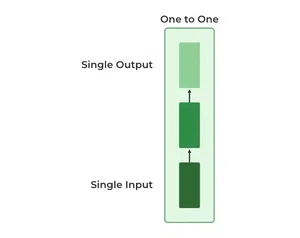
\includegraphics[
        width=\linewidth,
        height=2cm,
        keepaspectratio,
    ]{images/recurrent-neural-networks/rnn-gfg-5-One-to-One.png}
\end{figure}
\end{minipage}
\begin{minipage}{0.75\linewidth}
    \textbf{One-to-One RNN}: This is the simplest type of neural network architecture where there is a single input and a single output. It is used for straightforward classification tasks such as binary classification where no sequential data is involved.
    \hfill \cite{geeksforgeeks/machine-learning/introduction-to-recurrent-neural-network}
\end{minipage}
\end{table}

\begin{table}[H]
\begin{minipage}{0.2\linewidth}
\begin{figure}[H]
    \centering
    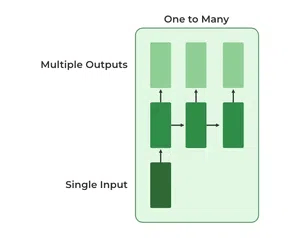
\includegraphics[
        width=\linewidth,
        height=2cm,
        keepaspectratio,
    ]{images/recurrent-neural-networks/rnn-gfg-6-One-to-Many.png}
\end{figure}
\end{minipage}
\begin{minipage}{0.75\linewidth}
    \textbf{One-to-Many RNN}: In a One-to-Many RNN the network processes a single input to produce multiple outputs over time. This is useful in tasks where one input triggers a sequence of predictions (outputs). For example in image captioning a single image can be used as input to generate a sequence of words as a caption.
    \hfill \cite{geeksforgeeks/machine-learning/introduction-to-recurrent-neural-network}
\end{minipage}
\end{table}

\begin{table}[H]
\begin{minipage}{0.2\linewidth}
\begin{figure}[H]
    \centering
    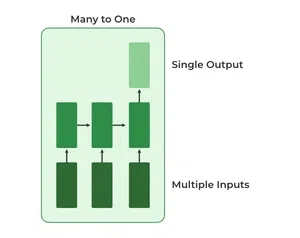
\includegraphics[
        width=\linewidth,
        height=2cm,
        keepaspectratio,
    ]{images/recurrent-neural-networks/rnn-gfg-7-Many-to-One.png}
\end{figure}
\end{minipage}
\begin{minipage}{0.75\linewidth}
    \textbf{Many-to-One RNN}: The Many-to-One RNN receives a sequence of inputs and generates a single output. This type is useful when the overall context of the input sequence is needed to make one prediction. In sentiment analysis the model receives a sequence of words (like a sentence) and produces a single output like positive, negative or neutral.
    \hfill \cite{geeksforgeeks/machine-learning/introduction-to-recurrent-neural-network}
\end{minipage}
\end{table}

\begin{table}[H]
\begin{minipage}{0.2\linewidth}
\begin{figure}[H]
    \centering
    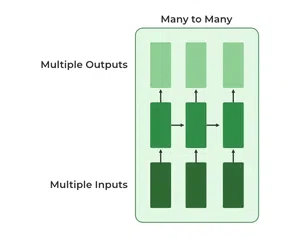
\includegraphics[
        width=\linewidth,
        height=2cm,
        keepaspectratio,
    ]{images/recurrent-neural-networks/rnn-gfg-8-Many-to-Many.png}
\end{figure}
\end{minipage}
\begin{minipage}{0.75\linewidth}
    \textbf{Many-to-Many RNN}: The Many-to-Many RNN type processes a sequence of inputs and generates a sequence of outputs. In language translation task a sequence of words in one language is given as input and a corresponding sequence in another language is generated as output.
    \hfill \cite{geeksforgeeks/machine-learning/introduction-to-recurrent-neural-network}
\end{minipage}
\end{table}





\section{Variants of Recurrent Neural Networks (RNNs)}

\begin{enumerate}
    \item \textbf{Vanilla RNN}: This \textbf{simplest} form of RNN consists of a single hidden layer where weights are shared across time steps. 
    Vanilla RNNs are suitable for learning short-term dependencies but are limited by the vanishing gradient problem, which hampers long-sequence learning.
    \hfill \cite{geeksforgeeks/machine-learning/introduction-to-recurrent-neural-network}
    

    \item \textbf{Bidirectional RNNs}: Bidirectional RNNs process inputs in both forward and backward directions, capturing both \textbf{past and future context} for each time step. 
    This architecture is ideal for tasks where the entire sequence is available, such as named entity recognition and question answering.
    \hfill \cite{geeksforgeeks/machine-learning/introduction-to-recurrent-neural-network}

    \item \textbf{Long Short-Term Memory Networks (LSTMs)}: Long Short-Term Memory Networks (LSTMs) introduce a memory mechanism to overcome the vanishing gradient problem. 
    Each LSTM cell has three gates:
    \hfill \cite{geeksforgeeks/machine-learning/introduction-to-recurrent-neural-network}
    \begin{enumerate}
        \item \textbf{Input Gate}: Controls how much new information should be added to the cell state.
        \hfill \cite{geeksforgeeks/machine-learning/introduction-to-recurrent-neural-network}
    
        \item \textbf{Forget Gate}: Decides what past information should be discarded.
        \hfill \cite{geeksforgeeks/machine-learning/introduction-to-recurrent-neural-network}
    
        \item \textbf{Output Gate}: Regulates what information should be output at the current step. This selective memory enables LSTMs to handle long-term dependencies, making them ideal for tasks where earlier context is critical.
        \hfill \cite{geeksforgeeks/machine-learning/introduction-to-recurrent-neural-network}
    \end{enumerate}

    \item \textbf{Gated Recurrent Units (GRUs)}: Gated Recurrent Units (GRUs) \textbf{simplify LSTMs} by combining the input and forget gates into a single update gate and streamlining the output mechanism. 
    This design is computationally efficient, often performing similarly to LSTMs and is useful in tasks where simplicity and faster training are beneficial.
    \hfill \cite{geeksforgeeks/machine-learning/introduction-to-recurrent-neural-network}
\end{enumerate}



\section{Disadvantages}

\begin{enumerate}
    \item Recurrent models typically factor computation along the symbol positions of the input and output sequences. 
    Aligning the positions to steps in computation time, they generate a sequence of hidden states $h_t$, as a function of the previous hidden state $h_{t-1}$ and the input for position $t$. 
    This inherently sequential nature precludes parallelization within training examples, which becomes critical at longer sequence lengths, as memory constraints limit batching across examples.
    \hfill \cite{arxiv/1706.03762/Attention-Is-All-You-Need}

    \item  RNNs traditionally require a pre-defined alignment between the input and output sequences to perform transduction. 
    This is a severe limitation since finding the alignment is the most difficult aspect of many sequence transduction problems. 
    \hfill \cite{arxiv/1211.3711/Sequence-Transduction-RNN}

    \item traditional RNNs face challenges such as the \textbf{vanishing gradient} problem where gradients become too small during backpropagation making training difficult.
    \hfill \cite{geeksforgeeks/deep-learning/bidirectional-recurrent-neural-network}
\end{enumerate}
















